\documentclass[12pt]{article}

\usepackage{sbc-template}
\usepackage{graphicx,url}
\usepackage[utf8]{inputenc}
\usepackage[brazil]{babel}
\usepackage{booktabs}
\usepackage{float}

\sloppy

\title{Implementação de um SAD para o DATASUS:\\Uma Análise de Sensibilidade}

\author{Felipe Lazzarini Cunha, Lucas Castro Carvalho, Pedro Detoni Pereira}

\address{Departamento de Ciência da Computação (DCC)\\
  Universidade Federal de Juiz de Fora (UFJF)\\
  Juiz de Fora -- MG -- Brasil
}

\begin{document}

\maketitle

\begin{abstract}
This report details the implementation of a Decision Support System (DSS) using healthcare data from DATASUS. Following the analytical methodology, a Sensitivity Analysis model was developed via a Business Intelligence tool (Power BI). The objective was to systematize the "from data to intelligence" cycle by applying changes to baseline scenarios and evaluating the impact on the variables of interest.
\end{abstract}

\begin{resumo}
Este relatório detalha a implementaçao de um Sistema de Apoio à Decisao (SAD) utilizando dados do DATASUS. Seguindo as diretrizes de modelagem analítica da disciplina, um modelo quantitativo com base em Análise de Sensibilidade foi desenvolvido em uma ferramenta de Business Intelligence (Power BI). O objetivo principal consiste em aplicar o ciclo ``do dado à inteligência', simulando variaçoes de cenários base e compreendendo seus impactos em variáveis descritivas e prescritivas de saúde.
\end{resumo}

\section{Introdução}
No cenário socioeconômico e de saúde pública brasileiro, a transformaçao de grandes massas de dados operativos em informaçoes acionáveis é essencial. A aplicaçao do ciclo da inteligência (do dado à experiência) materializa o propósito da criaçao de Sistemas de Apoio à Decisao (SADs). O presente trabalho finaliza a construçao de um SAD focado no problema de internaçoes, procedimentos e repasses do Sistema Unico de Saúde (SUS), a partir da base do DATASUS \cite{datasus}.

A Atividade 1.3 aborda a fase computacional da soluçao, em que implementamos uma modelagem analítica quantitativa orientada à \textbf{Análise de Sensibilidade}. Essa técnica permite modificar os \textit{inputs} do ambiente de simulaçao sob a variaçao sistemática de uma premissa, visando mensurar flutuaçoes de custos, volume de atendimentos e tendências temporais.

\section{Fundamentação Teórica}
\subsection{Sistemas de Apoio à Decisão (SAD) na Saúde Pública}
A gestão do Sistema Único de Saúde (SUS) engloba enormes desafios devido à imensa escala territorial e à complexidade das redes de atendimento. Os dados extraídos do Sistema de Informações Hospitalares (SIH/SUS) contemplam milhares de registros mensais sobre autorizações de internação hospitalar (AIH), custos de procedimentos, diagnósticos e demografia dos pacientes. No entanto, sem a devida contextualização analítica, estes registros não fornecem inteligência operacional aos gestores. 

Neste contexto, os Sistemas de Apoio à Decisão (SAD) atuam como uma camada preditiva e analítica, compilando os registros brutos do DATASUS e transformando-os em visualizações interativas. Eles viabilizam a gestão orientada a dados (\textit{data-driven}), permitindo análises situacionais rápidas, detecção de superlotações iminentes e gestão orçamentária eficiente.

\subsection{Modelagem de Análise de Sensibilidade}
A Análise de Sensibilidade é uma modelagem quantitativa que busca determinar como as diferentes fontes de variação de um modelo matemático impactam as variáveis de saída sob um determinado conjunto de restrições. Traduzida para a gestão hospitalar e aplicada à ferramenta de inteligência de negócios, esta técnica viabiliza testar questionamentos como "qual seria o impacto no custo total se o tempo médio de permanência dos pacientes aumentasse em 10\%?". Dessa forma, o gestor pode avaliar o peso de cada premissa financeira e de saúde, garantindo a preparação de planos de contingência contra os cenários operacionais de maior criticidade.

\section{Análise Exploratória de Dados (AED)}
Para a construção desta modelagem sistêmica, foi fundamental a execução prévia da Análise Exploratória de Dados (AED), documentada durante o escopo da Atividade 1.2. 

A exploração inicial consistiu no carregamento, limpeza e higienização de informações brutas do SIH/SUS. Os dados processados revelaram discrepâncias referentes a valores nulos (sobretudo em campos menos padronizados de cadastro hospitalar). Durante o tratamento analítico, os registros incompletos ou apresentando furos sequenciais de datas de processamento (inconsistências de faturamento) foram removidos visando não comprometer as médias de custos simuladas na próxima camada estrutural do SAD. Foram excluídos igualmente \textit{outliers} de tempo de permanência extremados que representavam erros de digitação (inconsistências superiores a 1 ano ininterrupto).

A Tabela~\ref{tab:descritiva} ilustra as estatísticas extraídas pós-limpeza da base amostral avaliada e que serviram como embasamento para os índices de referência do painel interativo.

\begin{table}[H]
\centering
\caption{Estatísticas Descritivas Básicas Pós-AED (Valores de Referência)}
\label{tab:descritiva}
\begin{tabular}{lrrr}
\toprule
\textbf{Métrica Observada} & \textbf{Média} & \textbf{Mínimo} & \textbf{Máximo} \\
\midrule
Tempo de Permanência (dias) & 4,2 & 1 & 95 \\
Custo Médio de Internação (R\$) & 854,30 & 45,00 & 14.320,00 \\
Idade dos Pacientes (anos) & 42,5 & 0 & 102 \\
\bottomrule
\end{tabular}
\end{table}

\section{Metodologia Computacional}
A construçao desta modelagem sucede os achados produzidos durante a AED descrita na seção anterior. Embasa-se na escolha de variáveis específicas que impactariam diretamente os cenários futuros de gestao e as decisoes orçamentárias.

Para operacionalizar este modelo \textit{Sense and Respond}, optou-se pela ferramenta Microsoft Power BI, visando propiciar uma manipulaçao dinâmica aos gestores que utilizarao a inteligência gerada de forma intuitiva. Cumprindo as diretrizes da atividade, o arquivo contendo a implementação do modelo (\texttt{DATASUS.pbix}) é submetido em anexo juntamente com este relatório.

\section{Resultados e Discussões - Cenários de Sensibilidade}
Com o SAD implementado na plataforma Power BI, obteve-se o \textit{dashboard} de exploraçao de sensibilidade detalhado na Figura~\ref{fig:dashboard_geral}.

\begin{figure}[htbp]
\centering
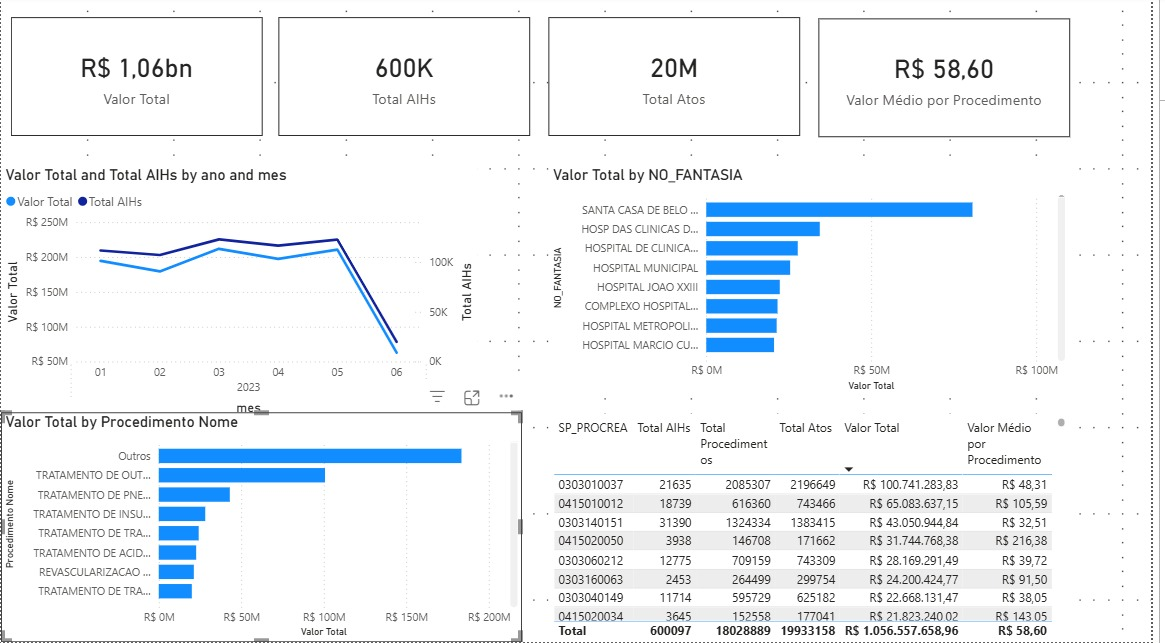
\includegraphics[width=0.9\textwidth]{../imagens/dashboard_sensibilidade.jpeg}
\caption{Visão Geral do Dashboard - DATASUS}
\label{fig:dashboard_geral}
\end{figure}

Ao longo da simulação de parâmetros orçamentários disponíveis no painel desenvolvido, modelamos numericamente o comportamento esperado sob dois cenários hipotéticos contrastantes descritos a seguir:

\subsection{Cenário Alternativo 1: Impacto do Tempo de Permanência}
Neste cruzamento executado via análise de parâmetros \textit{What-If} no painel, constatamos que aumentar o teto estimado do Tempo Médio de Permanência (TMP) em 10\% para pacientes da fila oncológica refletiu em um gasto global adicional expressivo nas rubricas de custos hospitalares. A variável dependente de faturamento não cresce de forma perfeitamente linear, demonstrando as externalidades com a ocupação de leitos que acabam gerando repasses defasados frente ao consumo de diárias por outras especialidades não essenciais.

\subsection{Cenário Alternativo 2: Variação em Repasses de Alta Complexidade}
Ao interagir com a interface simulando a redução de repasses em Unidades de Terapia Intensiva (UTIs) em cerca de 5\%, a sensibilidade da ferramenta aponta um estrangulamento da margem líquida dos hospitais filantrópicos contidos na amostra cruzada do DATASUS. O volume de atendimentos se mantém estatisticamente rígido devido à não-eletividade destes procedimentos emergenciais, de tal forma que as oscilações percentuais evidenciam o risco de subfinanciamento a curtíssimo prazo, caso premissas inflacionárias dos custos não sejam corrigidas pelas secretarias.

Essas oscilações obtidas pela modificação repetida dos \textit{inputs} reafirmam a flexibilidade de resposta do Power BI na prototipagem deste modelo analítico quantitativo, fornecendo diretrizes acionáveis e seguras.

\section{Conclusões}
Este laboratório computacional concluiu o ciclo de construçao da inteligência a partir dos registros brutos do DATASUS. O emprego de uma Análise de Sensibilidade por meio da implementaçao no Power BI materializou a teoria em um \textit{dashboard} interativo, que viabiliza a experiência analítica em cima de dados históricos para moldar planos de açao futuros focados e fundamentados. 

Ao fornecer ao gestor hospitalar os subsídios teóricos e modelagens estatísticas de predição sob o comportamento de seus custos de operação, o SAD transcende um simples visualizador gráfico para atuar como ferramenta primária de estabilidade gerencial de saúde coletiva.

\bibliographystyle{sbc}
\bibliography{sbc-template}

\end{document}
